\section{\method{} with Stochastic Value Gradients}
\label{sec:method}
We now introduce the SVG-based actor-critic variants, which differentiate the chain itself, avoiding the noise factor $\varepsilon_{k,i}^{\top}/\sigma_k$ in \methodGRPO{}. Each state in~(\ref{eq:chain}) is a differentiable function of the parameters and sampled noise, but the terminal reward has zero gradient almost everywhere because it depends on decoder $\arg\max$ and program verification. State value~(\ref{eq:value}) avoids this obstruction: \methodSVGScalar{} and \methodSVGTwoD{} learn differentiable value estimates $V_\phi$ and ascend them through one sampled transition.

\begin{figure}[t]
\centering
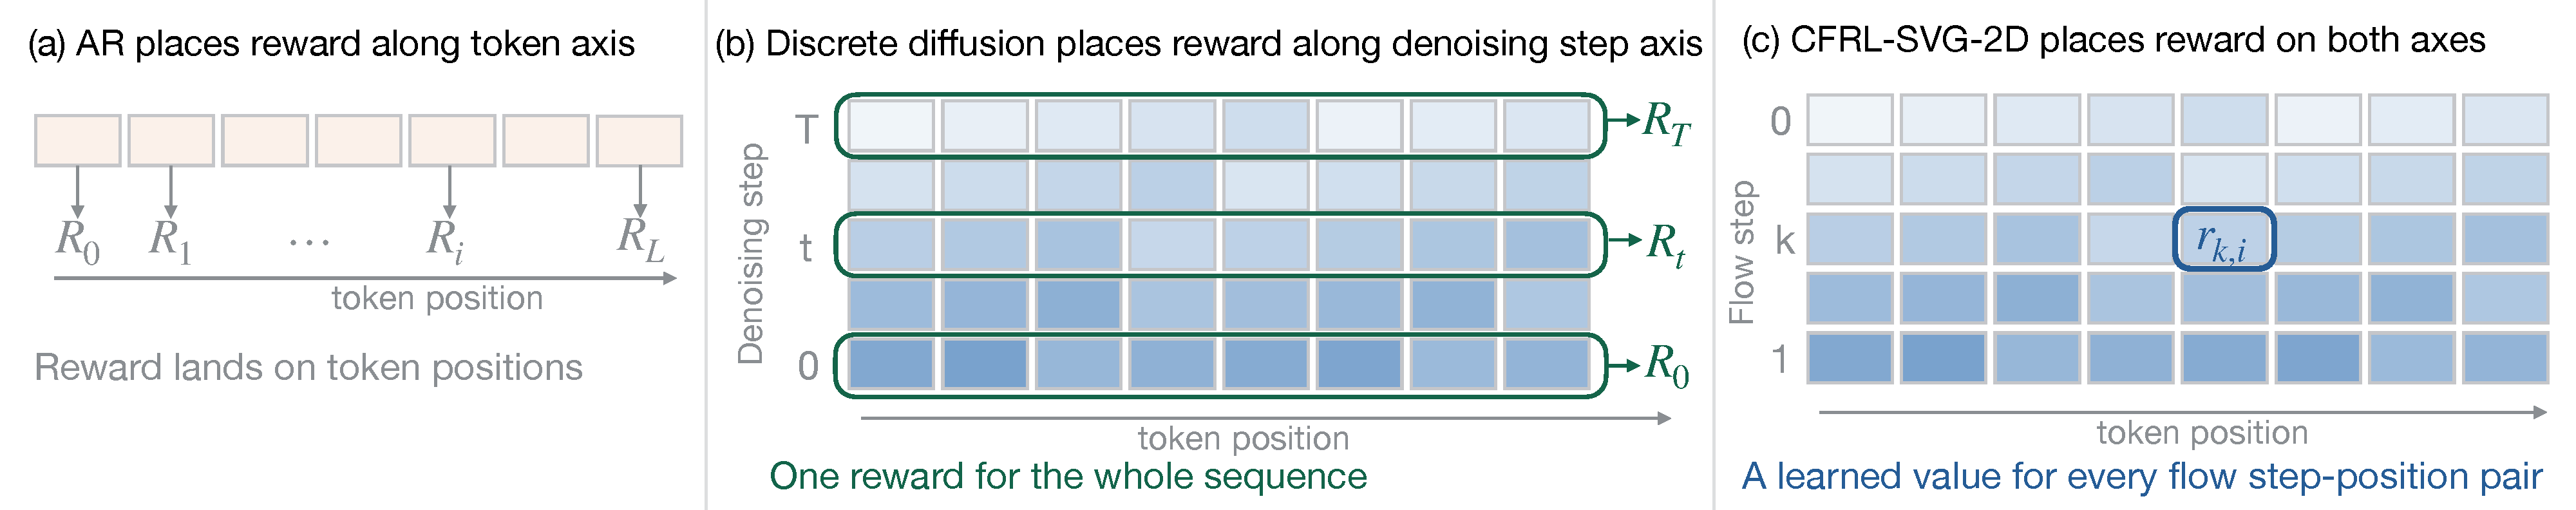
\includegraphics[width=\textwidth]{figures/flow-rl-figure1.pdf}
\caption{Where the reward lands. (a) In an AR model the reward is assigned along the token axis. (b) For discrete diffusion models it is assigned along the denoising-step axis. (c) Our 2D critic assigns a value $R_{k,i}$ to every flow step $k$ and position $i$.}
\label{fig:mechanism}
\end{figure}

\paragraph{Transition-wise value-gradient decomposition.}
The true value $V_k^*(y_k)$ summarizes the expected reward of all continuations from $y_k$. Unrolling the standard stochastic value-gradient (SVG) recursion \citep{heess2015svg} then decomposes the policy gradient into transition-wise contributions. Temporarily assigning transition $k$ its own parameter copy $\theta_k$, tied across steps after differentiation:
\begin{equation}
\label{eq:pw_exact}
\nabla_\theta J
=
\sum_{k=2}^{K-1}\frac{\partial J}{\partial\theta_k},
\qquad
\frac{\partial J}{\partial\theta_k}
= 
\mathbb E_{y_{k-1},\,\varepsilon_k}\!\left[
\alpha_k
\nabla_{y_k}V_k^*(y_k)^\top
\frac{\partial D_{\theta_k}(y_{k-1})}{\partial\theta_k}
\right].
\end{equation}
Sampling one transition estimates this sum up to a constant factor and consequently avoids back-propagation through the full chain. Gaussian integration by parts shows that this expression has the same expectation as its score-function counterpart (Appendix~\ref{app:pw_derivation}). At coordinate $(k,i)$, the score-function factor is $V_k^*(y_k)\varepsilon_{k,i}/\sigma_k$, which is noisy at every coordinate, whereas the pathwise factor is $\partial V_k^*(y_k)/\partial y_{k,i}$, which vanishes wherever the value is locally insensitive.


% JPC replaces $V^*$ in Eq~\ref{eq:pw_exact} by a critic that is trained with BCE loss, so its raw output approximates the log-odds of success $V_\phi(s_k)\approx\mathrm{logit}\,V(s_k)$. Accordingly, \jpc{} ascends
% \begin{equation}
% \tilde J_k(\theta)
% =
% \mathbb E\!\left[\mathrm{logit}\,V(s_k)\right],
% \qquad
% \nabla_{\theta_k}\mathrm{logit}\,V(s_k)
% =
% \frac{\nabla_{\theta_k}V(s_k)}
%      {V(s_k)(1-V(s_k))}.
% \label{eq:logodds}
% \end{equation}
% Thus, the log-odds and reward gradients have the same direction at each state but weight states differently. We use the log-odds because it is the scale learned directly by the BCE-trained critic.

\paragraph{Single-transition actor update.}
We sample $k\sim\mathcal U(\mathcal W)$ from a window
$\mathcal W=\{k_{\rm lo},\dots,k_{\rm hi}\}$ and use $\hat g_{\rm PW}=\nabla_\theta V_\phi(y_k)$. With an exact critic, its expectation is the window-averaged transition gradient. We use the middle of the chain, excluding early states with nearly flat values and late states whose outcomes are nearly determined. 

\subsection{\methodSVGScalar{}: a scalar critic on the flow state}
\label{sec:jpc_scalar}

\paragraph{Critic network.}
Predicting success from a noisy state requires anticipating its decoded output, which the denoiser already does. The critic therefore uses a separate copy $\hat D_\phi$ of the policy denoiser, initialized from $\hat D_\theta$ and evaluated without guidance, to read the input $y_k$ and $\tilde t_k$. Its per-position feature is $f_i(y_k)$ and the scalar critic pools these features before applying a time-conditioned head:
\begin{equation}
f_i(y_k)
=
\hat D_\phi(y_k,\tilde t_k)_i
\in\mathbb R^d,
\quad i\in\mathcal G, 
\quad V_\phi(y_k)
=
h_\phi\!\left(
\frac{1}{|\mathcal G|}
\sum_{i\in\mathcal G}f_i(y_k),
\tilde t_k
\right).
\label{eq:critic1d}
% \label{eq:feat}
\end{equation}
Because the transformer attends to the prompt and all sequence positions, each $f_i$ represents position $i$ in the context of the complete state. 

\paragraph{Training target.}
Each stored intermediate state is paired with its rollout's terminal outcome, so no intermediate labels are required. We train the critic by
\begin{equation}
\mathcal L_{\rm V}(\phi)
=
\mathbb E\!\left[
\mathrm{BCE}\bigl(V_\phi(y_k),r\bigr)
\right].
\label{eq:bce}
\end{equation}
Before RL, the denoiser copy and head are pretrained jointly on rollouts of the initial policy; during RL, the copy is frozen and only the head is updated with the policy (\S\ref{sec:joint}; Appendix~\ref{app:details}).

\subsection{\methodSVGTwoD{}: a critic over position and flow step}
\label{sec:jpc_2d}
\paragraph{2D critic.}
We propose a 2D critic motivated by the two-axis structure of flow generation: each state lies on a grid of flow steps and token positions (Figure~\ref{fig:mechanism}). AR methods index credit by token position, whereas diffusion and flow methods index it by denoising step and treat the full sequence state as one action \citep{liu2025flowgrpo,xue2025dancegrpo}. The scalar critic retains only the flow-step axis by pooling position features before value estimation. Our 2D critic restores the position axis by applying the value head before pooling:
\begin{equation}
R_{k,i}
=
h_\phi\bigl(f_i(y_k),\tilde t_k\bigr),
\qquad
V_\phi(y_k)
=
\frac{1}{|\mathcal G|}
\sum_{i\in\mathcal G}R_{k,i}.
\label{eq:critic2d}
\end{equation}
Each $R_{k,i}$ reads the outcome log-odds from position $i$, while their mean is the value ascended by the actor. The features and training procedure are unchanged from \methodSVGScalar{}. With the 2D critic, \emph{every position is pushed along its own direction.} By the chain rule the actor's signal at position $i$ is $\sum_{j\in\mathcal G}(\partial V_\phi/\partial f_j)(\partial f_j/\partial y_{k,i})$. The scalar critic applies the same head gradient to every position, whereas the 2D critic evaluates the head at each position's feature:
\begin{equation}
\text{head after the mean: }\ \frac{\partial V_\phi}{\partial f_j}=\frac{\nabla h_\phi(\mathrm{mean}(f))}{|\mathcal G|}\ ,\quad \text{head before the mean: }\ \frac{\partial V_\phi}{\partial f_j}=\frac{\nabla h_\phi(f_j)}{|\mathcal G|}.
\label{eq:headgrad}
\end{equation}
Thus, the scalar critic pushes all position features in one direction, while the 2D critic gives each position its own direction. The transformer may still couple positions through its Jacobian; the distinction lies in the signal assigned to each feature. The 2D critic also permits nonlinear dependence on each position feature, whereas a head on the mean can combine position contributions only affinely (Proposition~\ref{prop:additive}).

\emph{Outcome-supervised position values.} Both the pooled value and per-position readings are trained from the same terminal outcome:
\begin{equation}
\mathcal L_{\rm 2D}(\phi)=\tfrac12\,\mathrm{BCE}\bigl(V_\phi(y_k),r\bigr)+\tfrac12\,\frac1{|\mathcal G|}\sum_{i\in\mathcal G}\mathrm{BCE}\bigl(R_{k,i},r\bigr).
\label{eq:critic2d_loss}
\end{equation}
The second term provides no token-correctness labels; it calibrates each position's reading of sequence-level success, preventing the field from drifting while preserving its mean.

\subsection{Joint policy--critic training}
\label{sec:joint}
% Replacing the true log-odds with the learned critic introduces the gradient bias
% \begin{equation}
% \mathbb E\big[\nabla_\theta\,(V_\phi-\mathrm{logit}\,V)(y_k)\big],
% \label{eq:biasm}
% \end{equation}
% which vanishes when their slopes agree on states visited by the current policy. 
We update the critic jointly with the policy because as the policy changes, both states and their true values change, allowing a stale critic to be exploited. After each actor update, fresh rollouts are decoded and verified, and their states at $k_{\rm hi}$ are added with their outcomes to a recent replay buffer. We update the critic head on buffer minibatches, and the denoiser copy remains frozen. Because values depend on the sampling chain, actor and critic are trained under the sampler used for final evaluation, which we call the deployment sampler. Algorithm~\ref{alg:jpc} summarizes the procedure; further details appear in Appendix~\ref{app:details}.

